\documentclass[1p]{elsarticle_modified}
%\bibliographystyle{elsarticle-num}

%\usepackage[colorlinks]{hyperref}
%\usepackage{abbrmath_seonhwa} %\Abb, \Ascr, \Acal ,\Abf, \Afrak
\usepackage{amsfonts}
\usepackage{amssymb}
\usepackage{amsmath}
\usepackage{amsthm}
\usepackage{scalefnt}
\usepackage{amsbsy}
\usepackage{kotex}
\usepackage{caption}
\usepackage{subfig}
\usepackage{color}
\usepackage{graphicx}
\usepackage{xcolor} %% white, black, red, green, blue, cyan, magenta, yellow
\usepackage{float}
\usepackage{setspace}
\usepackage{hyperref}

\usepackage{tikz}
\usetikzlibrary{arrows}

\usepackage{multirow}
\usepackage{array} % fixed length table
\usepackage{hhline}

%%%%%%%%%%%%%%%%%%%%%
\makeatletter
\renewcommand*\env@matrix[1][\arraystretch]{%
	\edef\arraystretch{#1}%
	\hskip -\arraycolsep
	\let\@ifnextchar\new@ifnextchar
	\array{*\c@MaxMatrixCols c}}
\makeatother %https://tex.stackexchange.com/questions/14071/how-can-i-increase-the-line-spacing-in-a-matrix
%%%%%%%%%%%%%%%

\usepackage[normalem]{ulem}

\newcommand{\msout}[1]{\ifmmode\text{\sout{\ensuremath{#1}}}\else\sout{#1}\fi}
%SOURCE: \msout is \stkout macro in https://tex.stackexchange.com/questions/20609/strikeout-in-math-mode

\newcommand{\cancel}[1]{
	\ifmmode
	{\color{red}\msout{#1}}
	\else
	{\color{red}\sout{#1}}
	\fi
}

\newcommand{\add}[1]{
	{\color{blue}\uwave{#1}}
}

\newcommand{\replace}[2]{
	\ifmmode
	{\color{red}\msout{#1}}{\color{blue}\uwave{#2}}
	\else
	{\color{red}\sout{#1}}{\color{blue}\uwave{#2}}
	\fi
}

\newcommand{\Sol}{\mathcal{S}} %segment
\newcommand{\D}{D} %diagram
\newcommand{\A}{\mathcal{A}} %arc


%%%%%%%%%%%%%%%%%%%%%%%%%%%%%5 test

\def\sl{\operatorname{\textup{SL}}(2,\Cbb)}
\def\psl{\operatorname{\textup{PSL}}(2,\Cbb)}
\def\quan{\mkern 1mu \triangleright \mkern 1mu}

\theoremstyle{definition}
\newtheorem{thm}{Theorem}[section]
\newtheorem{prop}[thm]{Proposition}
\newtheorem{lem}[thm]{Lemma}
\newtheorem{ques}[thm]{Question}
\newtheorem{cor}[thm]{Corollary}
\newtheorem{defn}[thm]{Definition}
\newtheorem{exam}[thm]{Example}
\newtheorem{rmk}[thm]{Remark}
\newtheorem{alg}[thm]{Algorithm}

\newcommand{\I}{\sqrt{-1}}
\begin{document}

%\begin{frontmatter}
%
%\title{Boundary parabolic representations of knots up to 8 crossings}
%
%%% Group authors per affiliation:
%\author{Yunhi Cho} 
%\address{Department of Mathematics, University of Seoul, Seoul, Korea}
%\ead{yhcho@uos.ac.kr}
%
%
%\author{Seonhwa Kim} %\fnref{s_kim}}
%\address{Center for Geometry and Physics, Institute for Basic Science, Pohang, 37673, Korea}
%\ead{ryeona17@ibs.re.kr}
%
%\author{Hyuk Kim}
%\address{Department of Mathematical Sciences, Seoul National University, Seoul 08826, Korea}
%\ead{hyukkim@snu.ac.kr}
%
%\author{Seokbeom Yoon}
%\address{Department of Mathematical Sciences, Seoul National University, Seoul, 08826,  Korea}
%\ead{sbyoon15@snu.ac.kr}
%
%\begin{abstract}
%We find all boundary parabolic representation of knots up to 8 crossings.
%
%\end{abstract}
%\begin{keyword}
%    \MSC[2010] 57M25 
%\end{keyword}
%
%\end{frontmatter}

%\linenumbers
%\tableofcontents
%
\newcommand\colored[1]{\textcolor{white}{\rule[-0.35ex]{0.8em}{1.4ex}}\kern-0.8em\color{red} #1}%
%\newcommand\colored[1]{\textcolor{white}{ #1}\kern-2.17ex	\textcolor{white}{ #1}\kern-1.81ex	\textcolor{white}{ #1}\kern-2.15ex\color{red}#1	}

{\Large $\underline{12n_{0727}~(K12n_{0727})}$}

\setlength{\tabcolsep}{10pt}
\renewcommand{\arraystretch}{1.6}
\vspace{1cm}\begin{tabular}{m{100pt}>{\centering\arraybackslash}m{274pt}}
\multirow{5}{120pt}{
	\centering
	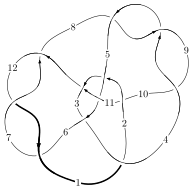
\includegraphics[width=112pt]{../../../GIT/diagram.site/Diagrams/png/2816_12n_0727.png}\\
\ \ \ A knot diagram\footnotemark}&
\allowdisplaybreaks
\textbf{Linearized knot diagam} \\
\cline{2-2}
 &
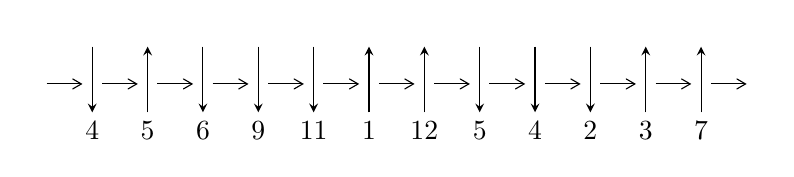
\begin{tikzpicture}[x=20pt, y=17pt]
	% nodes
	\node (C0) at (0, 0) {};
	\node (C1) at (1, 0) {};
	\node (C1U) at (1, +1) {};
	\node (C1D) at (1, -1) {4};

	\node (C2) at (2, 0) {};
	\node (C2U) at (2, +1) {};
	\node (C2D) at (2, -1) {5};

	\node (C3) at (3, 0) {};
	\node (C3U) at (3, +1) {};
	\node (C3D) at (3, -1) {6};

	\node (C4) at (4, 0) {};
	\node (C4U) at (4, +1) {};
	\node (C4D) at (4, -1) {9};

	\node (C5) at (5, 0) {};
	\node (C5U) at (5, +1) {};
	\node (C5D) at (5, -1) {11};

	\node (C6) at (6, 0) {};
	\node (C6U) at (6, +1) {};
	\node (C6D) at (6, -1) {1};

	\node (C7) at (7, 0) {};
	\node (C7U) at (7, +1) {};
	\node (C7D) at (7, -1) {12};

	\node (C8) at (8, 0) {};
	\node (C8U) at (8, +1) {};
	\node (C8D) at (8, -1) {5};

	\node (C9) at (9, 0) {};
	\node (C9U) at (9, +1) {};
	\node (C9D) at (9, -1) {4};

	\node (C10) at (10, 0) {};
	\node (C10U) at (10, +1) {};
	\node (C10D) at (10, -1) {2};

	\node (C11) at (11, 0) {};
	\node (C11U) at (11, +1) {};
	\node (C11D) at (11, -1) {3};

	\node (C12) at (12, 0) {};
	\node (C12U) at (12, +1) {};
	\node (C12D) at (12, -1) {7};
	\node (C13) at (13, 0) {};

	% arrows
	\draw[->,>={angle 60}]
	(C0) edge (C1) (C1) edge (C2) (C2) edge (C3) (C3) edge (C4) (C4) edge (C5) (C5) edge (C6) (C6) edge (C7) (C7) edge (C8) (C8) edge (C9) (C9) edge (C10) (C10) edge (C11) (C11) edge (C12) (C12) edge (C13) ;	\draw[->,>=stealth]
	(C1U) edge (C1D) (C2D) edge (C2U) (C3U) edge (C3D) (C4U) edge (C4D) (C5U) edge (C5D) (C6D) edge (C6U) (C7D) edge (C7U) (C8U) edge (C8D) (C9U) edge (C9D) (C10U) edge (C10D) (C11D) edge (C11U) (C12D) edge (C12U) ;
	\end{tikzpicture} \\
\hhline{~~} \\& 
\textbf{Solving Sequence} \\ \cline{2-2} 
 &
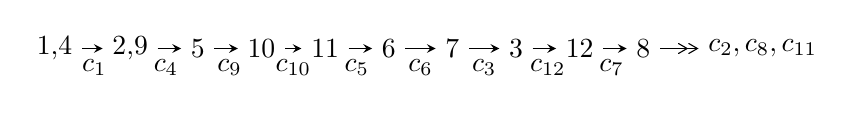
\begin{tikzpicture}[x=23pt, y=7pt]
	% node
	\node (A0) at (-1/8, 0) {1,4};
	\node (A1) at (17/16, 0) {2,9};
	\node (A2) at (17/8, 0) {5};
	\node (A3) at (25/8, 0) {10};
	\node (A4) at (33/8, 0) {11};
	\node (A5) at (41/8, 0) {6};
	\node (A6) at (49/8, 0) {7};
	\node (A7) at (57/8, 0) {3};
	\node (A8) at (65/8, 0) {12};
	\node (A9) at (73/8, 0) {8};
	\node (C1) at (1/2, -1) {$c_{1}$};
	\node (C2) at (13/8, -1) {$c_{4}$};
	\node (C3) at (21/8, -1) {$c_{9}$};
	\node (C4) at (29/8, -1) {$c_{10}$};
	\node (C5) at (37/8, -1) {$c_{5}$};
	\node (C6) at (45/8, -1) {$c_{6}$};
	\node (C7) at (53/8, -1) {$c_{3}$};
	\node (C8) at (61/8, -1) {$c_{12}$};
	\node (C9) at (69/8, -1) {$c_{7}$};
	\node (A10) at (11, 0) {$c_{2},c_{8},c_{11}$};

	% edge
	\draw[->,>=stealth]	
	(A0) edge (A1) (A1) edge (A2) (A2) edge (A3) (A3) edge (A4) (A4) edge (A5) (A5) edge (A6) (A6) edge (A7) (A7) edge (A8) (A8) edge (A9) ;
	\draw[->>,>={angle 60}]	
	(A9) edge (A10);
\end{tikzpicture} \\ 

\end{tabular} \\

\footnotetext{
The image of knot diagram is generated by the software ``\textbf{Draw programme}" developed by Andrew Bartholomew(\url{http://www.layer8.co.uk/maths/draw/index.htm\#Running-draw}), where we modified some parts for our purpose(\url{https://github.com/CATsTAILs/LinksPainter}).
}\phantom \\ \newline 
\centering \textbf{Ideals for irreducible components\footnotemark of $X_{\text{par}}$} 
 
\begin{align*}
I^u_{1}&=\langle 
-3.94440\times10^{300} u^{70}+2.53784\times10^{301} u^{69}+\cdots+3.21640\times10^{303} b+1.14997\times10^{304},\\
\phantom{I^u_{1}}&\phantom{= \langle  }-1.18258\times10^{304} u^{70}+7.69862\times10^{304} u^{69}+\cdots+3.29038\times10^{306} a+3.83134\times10^{307},\\
\phantom{I^u_{1}}&\phantom{= \langle  }u^{71}-6 u^{70}+\cdots-4114 u-1331\rangle \\
I^u_{2}&=\langle 
1.81727\times10^{28} u^{25}-2.58039\times10^{29} u^{24}+\cdots+1.41382\times10^{28} b-4.03240\times10^{29},\\
\phantom{I^u_{2}}&\phantom{= \langle  }7.46795\times10^{29} u^{25}-1.06112\times10^{31} u^{24}+\cdots+2.40350\times10^{29} a-1.63428\times10^{31},\\
\phantom{I^u_{2}}&\phantom{= \langle  }u^{26}-15 u^{25}+\cdots-101 u+17\rangle \\
\\
\end{align*}
\raggedright * 2 irreducible components of $\dim_{\mathbb{C}}=0$, with total 97 representations.\\
\footnotetext{All coefficients of polynomials are rational numbers. But the coefficients are sometimes approximated in decimal forms when there is not enough margin.}
\newpage
\renewcommand{\arraystretch}{1}
\centering \section*{I. $I^u_{1}= \langle -3.94\times10^{300} u^{70}+2.54\times10^{301} u^{69}+\cdots+3.22\times10^{303} b+1.15\times10^{304},\;-1.18\times10^{304} u^{70}+7.70\times10^{304} u^{69}+\cdots+3.29\times10^{306} a+3.83\times10^{307},\;u^{71}-6 u^{70}+\cdots-4114 u-1331 \rangle$}
\flushleft \textbf{(i) Arc colorings}\\
\begin{tabular}{m{7pt} m{180pt} m{7pt} m{180pt} }
\flushright $a_{1}=$&$\begin{pmatrix}1\\0\end{pmatrix}$ \\
\flushright $a_{4}=$&$\begin{pmatrix}0\\u\end{pmatrix}$ \\
\flushright $a_{2}=$&$\begin{pmatrix}1\\u^2\end{pmatrix}$ \\
\flushright $a_{9}=$&$\begin{pmatrix}0.00359405 u^{70}-0.0233974 u^{69}+\cdots-10.2765 u-11.6441\\0.00122634 u^{70}-0.00789030 u^{69}+\cdots-6.17758 u-3.57534\end{pmatrix}$ \\
\flushright $a_{5}=$&$\begin{pmatrix}0.00598596 u^{70}-0.0384900 u^{69}+\cdots-20.1705 u-18.3721\\-0.000291346 u^{70}+0.00211473 u^{69}+\cdots+2.72153 u+0.00758362\end{pmatrix}$ \\
\flushright $a_{10}=$&$\begin{pmatrix}0.00359405 u^{70}-0.0233974 u^{69}+\cdots-10.2765 u-11.6441\\0.00223421 u^{70}-0.0144905 u^{69}+\cdots-8.93510 u-6.01514\end{pmatrix}$ \\
\flushright $a_{11}=$&$\begin{pmatrix}0.00236772 u^{70}-0.0155071 u^{69}+\cdots-4.09892 u-8.06874\\0.00196736 u^{70}-0.0127690 u^{69}+\cdots-8.37761 u-5.30669\end{pmatrix}$ \\
\flushright $a_{6}=$&$\begin{pmatrix}0.000944024 u^{70}-0.00534102 u^{69}+\cdots+2.29413 u-4.92832\\-0.00266769 u^{70}+0.0173963 u^{69}+\cdots+10.1384 u+5.89187\end{pmatrix}$ \\
\flushright $a_{7}=$&$\begin{pmatrix}-0.00172367 u^{70}+0.0120553 u^{69}+\cdots+12.4325 u+0.963549\\-0.00266769 u^{70}+0.0173963 u^{69}+\cdots+10.1384 u+5.89187\end{pmatrix}$ \\
\flushright $a_{3}=$&$\begin{pmatrix}-0.00219214 u^{70}+0.0150659 u^{69}+\cdots+18.3981 u+2.02950\\-0.00416424 u^{70}+0.0270500 u^{69}+\cdots+13.2979 u+10.3819\end{pmatrix}$ \\
\flushright $a_{12}=$&$\begin{pmatrix}0.00900947 u^{70}-0.0586001 u^{69}+\cdots-17.8826 u-23.4781\\0.00120943 u^{70}-0.00763559 u^{69}+\cdots-2.89220 u-4.68656\end{pmatrix}$ \\
\flushright $a_{8}=$&$\begin{pmatrix}0.00145832 u^{70}-0.00974600 u^{69}+\cdots-2.07797 u-3.06258\\0.00371565 u^{70}-0.0241597 u^{69}+\cdots-10.5062 u-9.72889\end{pmatrix}$\\&\end{tabular}
\flushleft \textbf{(ii) Obstruction class $= -1$}\\~\\
\flushleft \textbf{(iii) Cusp Shapes $= 0.00212616 u^{70}-0.0143000 u^{69}+\cdots+4.47275 u-9.19315$}\\~\\
\newpage\renewcommand{\arraystretch}{1}
\flushleft \textbf{(iv) u-Polynomials at the component}\newline \\
\begin{tabular}{m{50pt}|m{274pt}}
Crossings & \hspace{64pt}u-Polynomials at each crossing \\
\hline $$\begin{aligned}c_{1}\end{aligned}$$&$\begin{aligned}
&u^{71}+6 u^{70}+\cdots-4114 u+1331
\end{aligned}$\\
\hline $$\begin{aligned}c_{2}\end{aligned}$$&$\begin{aligned}
&u^{71}+21 u^{69}+\cdots-83828 u+3624
\end{aligned}$\\
\hline $$\begin{aligned}c_{3}\end{aligned}$$&$\begin{aligned}
&u^{71}- u^{70}+\cdots-247794 u+25577
\end{aligned}$\\
\hline $$\begin{aligned}c_{4},c_{8},c_{9}\end{aligned}$$&$\begin{aligned}
&u^{71}+9 u^{69}+\cdots+19 u-1
\end{aligned}$\\
\hline $$\begin{aligned}c_{5}\end{aligned}$$&$\begin{aligned}
&u^{71}+u^{70}+\cdots-2 u+11
\end{aligned}$\\
\hline $$\begin{aligned}c_{6},c_{7},c_{12}\end{aligned}$$&$\begin{aligned}
&u^{71}+39 u^{69}+\cdots-5 u+27
\end{aligned}$\\
\hline $$\begin{aligned}c_{10}\end{aligned}$$&$\begin{aligned}
&u^{71}-34 u^{69}+\cdots+56160 u+8128
\end{aligned}$\\
\hline $$\begin{aligned}c_{11}\end{aligned}$$&$\begin{aligned}
&u^{71}-4 u^{70}+\cdots+1157 u+17
\end{aligned}$\\
\hline
\end{tabular}\\~\\
\newpage\renewcommand{\arraystretch}{1}
\flushleft \textbf{(v) Riley Polynomials at the component}\newline \\
\begin{tabular}{m{50pt}|m{274pt}}
Crossings & \hspace{64pt}Riley Polynomials at each crossing \\
\hline $$\begin{aligned}c_{1}\end{aligned}$$&$\begin{aligned}
&y^{71}-78 y^{70}+\cdots+1815484 y-1771561
\end{aligned}$\\
\hline $$\begin{aligned}c_{2}\end{aligned}$$&$\begin{aligned}
&y^{71}+42 y^{70}+\cdots+1092384208 y-13133376
\end{aligned}$\\
\hline $$\begin{aligned}c_{3}\end{aligned}$$&$\begin{aligned}
&y^{71}-23 y^{70}+\cdots+22971145086 y-654182929
\end{aligned}$\\
\hline $$\begin{aligned}c_{4},c_{8},c_{9}\end{aligned}$$&$\begin{aligned}
&y^{71}+18 y^{70}+\cdots+101 y-1
\end{aligned}$\\
\hline $$\begin{aligned}c_{5}\end{aligned}$$&$\begin{aligned}
&y^{71}-5 y^{70}+\cdots+4008 y-121
\end{aligned}$\\
\hline $$\begin{aligned}c_{6},c_{7},c_{12}\end{aligned}$$&$\begin{aligned}
&y^{71}+78 y^{70}+\cdots-65369 y-729
\end{aligned}$\\
\hline $$\begin{aligned}c_{10}\end{aligned}$$&$\begin{aligned}
&y^{71}-68 y^{70}+\cdots-2954669056 y-66064384
\end{aligned}$\\
\hline $$\begin{aligned}c_{11}\end{aligned}$$&$\begin{aligned}
&y^{71}+20 y^{70}+\cdots+471071 y-289
\end{aligned}$\\
\hline
\end{tabular}\\~\\
\newpage\flushleft \textbf{(vi) Complex Volumes and Cusp Shapes}
$$\begin{array}{c|c|c}  
\text{Solutions to }I^u_{1}& \I (\text{vol} + \sqrt{-1}CS) & \text{Cusp shape}\\
 \hline 
\begin{aligned}
u &= -0.855093 + 0.691769 I \\
a &= -0.819852 + 0.703890 I \\
b &= \phantom{-}0.751162 + 1.181190 I\end{aligned}
 & -4.12043 - 2.13457 I & \phantom{-0.000000 } 0 \\ \hline\begin{aligned}
u &= -0.855093 - 0.691769 I \\
a &= -0.819852 - 0.703890 I \\
b &= \phantom{-}0.751162 - 1.181190 I\end{aligned}
 & -4.12043 + 2.13457 I & \phantom{-0.000000 } 0 \\ \hline\begin{aligned}
u &= -0.945495 + 0.576536 I \\
a &= \phantom{-}0.383796 - 0.492811 I \\
b &= -0.313568 - 1.042450 I\end{aligned}
 & \phantom{-}1.80017 - 2.63067 I & \phantom{-0.000000 } 0 \\ \hline\begin{aligned}
u &= -0.945495 - 0.576536 I \\
a &= \phantom{-}0.383796 + 0.492811 I \\
b &= -0.313568 + 1.042450 I\end{aligned}
 & \phantom{-}1.80017 + 2.63067 I & \phantom{-0.000000 } 0 \\ \hline\begin{aligned}
u &= \phantom{-}0.410222 + 0.694548 I \\
a &= \phantom{-}0.629449 + 0.468517 I \\
b &= \phantom{-}0.892647 - 0.752338 I\end{aligned}
 & \phantom{-}1.07011 - 1.96163 I & \phantom{-}4.17135 + 0. I\phantom{ +0.000000I} \\ \hline\begin{aligned}
u &= \phantom{-}0.410222 - 0.694548 I \\
a &= \phantom{-}0.629449 - 0.468517 I \\
b &= \phantom{-}0.892647 + 0.752338 I\end{aligned}
 & \phantom{-}1.07011 + 1.96163 I & \phantom{-}4.17135 + 0. I\phantom{ +0.000000I} \\ \hline\begin{aligned}
u &= \phantom{-}0.710634 + 1.047830 I \\
a &= -0.754572 - 0.114387 I \\
b &= -0.168552 + 0.356847 I\end{aligned}
 & -4.75391 - 4.28782 I & \phantom{-0.000000 } 0 \\ \hline\begin{aligned}
u &= \phantom{-}0.710634 - 1.047830 I \\
a &= -0.754572 + 0.114387 I \\
b &= -0.168552 - 0.356847 I\end{aligned}
 & -4.75391 + 4.28782 I & \phantom{-0.000000 } 0 \\ \hline\begin{aligned}
u &= -0.722568 + 0.079323 I \\
a &= \phantom{-}0.05240 - 2.01983 I \\
b &= -0.108948 - 0.811922 I\end{aligned}
 & \phantom{-}5.63700 - 3.03551 I & \phantom{-}11.5234 - 18.6135 I \\ \hline\begin{aligned}
u &= -0.722568 - 0.079323 I \\
a &= \phantom{-}0.05240 + 2.01983 I \\
b &= -0.108948 + 0.811922 I\end{aligned}
 & \phantom{-}5.63700 + 3.03551 I & \phantom{-}11.5234 + 18.6135 I\\
 \hline 
 \end{array}$$\newpage$$\begin{array}{c|c|c}  
\text{Solutions to }I^u_{1}& \I (\text{vol} + \sqrt{-1}CS) & \text{Cusp shape}\\
 \hline 
\begin{aligned}
u &= \phantom{-}1.29924\phantom{ +0.000000I} \\
a &= -0.201632\phantom{ +0.000000I} \\
b &= -1.10829\phantom{ +0.000000I}\end{aligned}
 & -2.21745\phantom{ +0.000000I} & \phantom{-0.000000 } 0 \\ \hline\begin{aligned}
u &= \phantom{-}0.421745 + 0.482603 I \\
a &= \phantom{-}1.286390 - 0.505129 I \\
b &= \phantom{-}0.17570 + 2.03467 I\end{aligned}
 & -7.18912 - 6.23246 I & -7.19469 + 7.21845 I \\ \hline\begin{aligned}
u &= \phantom{-}0.421745 - 0.482603 I \\
a &= \phantom{-}1.286390 + 0.505129 I \\
b &= \phantom{-}0.17570 - 2.03467 I\end{aligned}
 & -7.18912 + 6.23246 I & -7.19469 - 7.21845 I \\ \hline\begin{aligned}
u &= -1.394060 + 0.131721 I \\
a &= \phantom{-}0.938577 - 0.467693 I \\
b &= \phantom{-}2.02334 - 0.02777 I\end{aligned}
 & -13.85970 - 0.07874 I & \phantom{-0.000000 } 0 \\ \hline\begin{aligned}
u &= -1.394060 - 0.131721 I \\
a &= \phantom{-}0.938577 + 0.467693 I \\
b &= \phantom{-}2.02334 + 0.02777 I\end{aligned}
 & -13.85970 + 0.07874 I & \phantom{-0.000000 } 0 \\ \hline\begin{aligned}
u &= \phantom{-}0.174970 + 0.540137 I \\
a &= \phantom{-}0.639636 - 0.981256 I \\
b &= -0.071320 - 0.148905 I\end{aligned}
 & -1.21580 - 0.98742 I & -6.40420 + 1.68200 I \\ \hline\begin{aligned}
u &= \phantom{-}0.174970 - 0.540137 I \\
a &= \phantom{-}0.639636 + 0.981256 I \\
b &= -0.071320 + 0.148905 I\end{aligned}
 & -1.21580 + 0.98742 I & -6.40420 - 1.68200 I \\ \hline\begin{aligned}
u &= \phantom{-}0.476772 + 0.258180 I \\
a &= -1.49190 + 1.16051 I \\
b &= \phantom{-}0.063631 + 0.926165 I\end{aligned}
 & -8.00321 + 1.13862 I & -8.21760 + 1.16511 I \\ \hline\begin{aligned}
u &= \phantom{-}0.476772 - 0.258180 I \\
a &= -1.49190 - 1.16051 I \\
b &= \phantom{-}0.063631 - 0.926165 I\end{aligned}
 & -8.00321 - 1.13862 I & -8.21760 - 1.16511 I \\ \hline\begin{aligned}
u &= -1.42761 + 0.39916 I \\
a &= -0.864889 + 0.393780 I \\
b &= -1.89045 + 0.33289 I\end{aligned}
 & -5.91928 + 4.99041 I & \phantom{-0.000000 } 0\\
 \hline 
 \end{array}$$\newpage$$\begin{array}{c|c|c}  
\text{Solutions to }I^u_{1}& \I (\text{vol} + \sqrt{-1}CS) & \text{Cusp shape}\\
 \hline 
\begin{aligned}
u &= -1.42761 - 0.39916 I \\
a &= -0.864889 - 0.393780 I \\
b &= -1.89045 - 0.33289 I\end{aligned}
 & -5.91928 - 4.99041 I & \phantom{-0.000000 } 0 \\ \hline\begin{aligned}
u &= -1.32126 + 0.67554 I \\
a &= \phantom{-}0.0726928 + 0.0562535 I \\
b &= \phantom{-}0.348804 + 0.734113 I\end{aligned}
 & -1.86664 - 2.54988 I & \phantom{-0.000000 } 0 \\ \hline\begin{aligned}
u &= -1.32126 - 0.67554 I \\
a &= \phantom{-}0.0726928 - 0.0562535 I \\
b &= \phantom{-}0.348804 - 0.734113 I\end{aligned}
 & -1.86664 + 2.54988 I & \phantom{-0.000000 } 0 \\ \hline\begin{aligned}
u &= -0.479123 + 0.152614 I \\
a &= -1.28987 + 0.59984 I \\
b &= -0.740321 + 0.170047 I\end{aligned}
 & -0.70765 + 1.68837 I & -1.63894 - 3.69018 I \\ \hline\begin{aligned}
u &= -0.479123 - 0.152614 I \\
a &= -1.28987 - 0.59984 I \\
b &= -0.740321 - 0.170047 I\end{aligned}
 & -0.70765 - 1.68837 I & -1.63894 + 3.69018 I \\ \hline\begin{aligned}
u &= \phantom{-}0.27206 + 1.47654 I \\
a &= -0.388494 + 0.277917 I \\
b &= -0.289408 - 0.266420 I\end{aligned}
 & \phantom{-}0.11277 - 4.26226 I & \phantom{-0.000000 } 0 \\ \hline\begin{aligned}
u &= \phantom{-}0.27206 - 1.47654 I \\
a &= -0.388494 - 0.277917 I \\
b &= -0.289408 + 0.266420 I\end{aligned}
 & \phantom{-}0.11277 + 4.26226 I & \phantom{-0.000000 } 0 \\ \hline\begin{aligned}
u &= -1.50420 + 0.03923 I \\
a &= -0.686049 + 0.733307 I \\
b &= -1.58379 + 0.51372 I\end{aligned}
 & -5.23867 + 2.59454 I & \phantom{-0.000000 } 0 \\ \hline\begin{aligned}
u &= -1.50420 - 0.03923 I \\
a &= -0.686049 - 0.733307 I \\
b &= -1.58379 - 0.51372 I\end{aligned}
 & -5.23867 - 2.59454 I & \phantom{-0.000000 } 0 \\ \hline\begin{aligned}
u &= -0.487748 + 0.064878 I \\
a &= \phantom{-}1.03010 - 3.02691 I \\
b &= -0.711670 - 0.570558 I\end{aligned}
 & -3.00603 + 4.33794 I & -5.75149 - 2.20133 I\\
 \hline 
 \end{array}$$\newpage$$\begin{array}{c|c|c}  
\text{Solutions to }I^u_{1}& \I (\text{vol} + \sqrt{-1}CS) & \text{Cusp shape}\\
 \hline 
\begin{aligned}
u &= -0.487748 - 0.064878 I \\
a &= \phantom{-}1.03010 + 3.02691 I \\
b &= -0.711670 + 0.570558 I\end{aligned}
 & -3.00603 - 4.33794 I & -5.75149 + 2.20133 I \\ \hline\begin{aligned}
u &= \phantom{-}1.47327 + 0.47471 I \\
a &= -0.938303 - 0.554952 I \\
b &= -1.58558 - 0.11609 I\end{aligned}
 & -10.53540 - 5.22803 I & \phantom{-0.000000 } 0 \\ \hline\begin{aligned}
u &= \phantom{-}1.47327 - 0.47471 I \\
a &= -0.938303 + 0.554952 I \\
b &= -1.58558 + 0.11609 I\end{aligned}
 & -10.53540 + 5.22803 I & \phantom{-0.000000 } 0 \\ \hline\begin{aligned}
u &= -1.56403 + 0.07841 I \\
a &= \phantom{-}0.649067 + 0.652560 I \\
b &= \phantom{-}1.61142 + 0.17827 I\end{aligned}
 & -6.26383 + 3.91447 I & \phantom{-0.000000 } 0 \\ \hline\begin{aligned}
u &= -1.56403 - 0.07841 I \\
a &= \phantom{-}0.649067 - 0.652560 I \\
b &= \phantom{-}1.61142 - 0.17827 I\end{aligned}
 & -6.26383 - 3.91447 I & \phantom{-0.000000 } 0 \\ \hline\begin{aligned}
u &= \phantom{-}0.382869 + 0.152364 I \\
a &= -0.700984 - 0.217875 I \\
b &= -0.16005 - 1.81276 I\end{aligned}
 & \phantom{-}0.89217 - 2.87299 I & -12.8712 + 10.4575 I \\ \hline\begin{aligned}
u &= \phantom{-}0.382869 - 0.152364 I \\
a &= -0.700984 + 0.217875 I \\
b &= -0.16005 + 1.81276 I\end{aligned}
 & \phantom{-}0.89217 + 2.87299 I & -12.8712 - 10.4575 I \\ \hline\begin{aligned}
u &= \phantom{-}0.148157 + 0.376556 I \\
a &= \phantom{-}1.93101 + 0.10965 I \\
b &= \phantom{-}0.023725 - 0.684740 I\end{aligned}
 & \phantom{-}0.53283 - 1.57625 I & -0.35637 + 4.67830 I \\ \hline\begin{aligned}
u &= \phantom{-}0.148157 - 0.376556 I \\
a &= \phantom{-}1.93101 - 0.10965 I \\
b &= \phantom{-}0.023725 + 0.684740 I\end{aligned}
 & \phantom{-}0.53283 + 1.57625 I & -0.35637 - 4.67830 I \\ \hline\begin{aligned}
u &= -1.59234 + 0.18903 I \\
a &= \phantom{-}0.687009 - 0.705876 I \\
b &= \phantom{-}1.62510 - 0.75960 I\end{aligned}
 & -12.3054 + 8.0119 I & \phantom{-0.000000 } 0\\
 \hline 
 \end{array}$$\newpage$$\begin{array}{c|c|c}  
\text{Solutions to }I^u_{1}& \I (\text{vol} + \sqrt{-1}CS) & \text{Cusp shape}\\
 \hline 
\begin{aligned}
u &= -1.59234 - 0.18903 I \\
a &= \phantom{-}0.687009 + 0.705876 I \\
b &= \phantom{-}1.62510 + 0.75960 I\end{aligned}
 & -12.3054 - 8.0119 I & \phantom{-0.000000 } 0 \\ \hline\begin{aligned}
u &= \phantom{-}1.10230 + 1.16672 I \\
a &= -0.466795 - 0.288870 I \\
b &= -1.165100 + 0.306719 I\end{aligned}
 & -4.13954 - 5.68269 I & \phantom{-0.000000 } 0 \\ \hline\begin{aligned}
u &= \phantom{-}1.10230 - 1.16672 I \\
a &= -0.466795 + 0.288870 I \\
b &= -1.165100 - 0.306719 I\end{aligned}
 & -4.13954 + 5.68269 I & \phantom{-0.000000 } 0 \\ \hline\begin{aligned}
u &= -1.61148 + 0.10779 I \\
a &= -0.756015 - 0.575680 I \\
b &= -1.88784 + 0.14386 I\end{aligned}
 & -14.5113 + 8.0913 I & \phantom{-0.000000 } 0 \\ \hline\begin{aligned}
u &= -1.61148 - 0.10779 I \\
a &= -0.756015 + 0.575680 I \\
b &= -1.88784 - 0.14386 I\end{aligned}
 & -14.5113 - 8.0913 I & \phantom{-0.000000 } 0 \\ \hline\begin{aligned}
u &= \phantom{-}1.46018 + 0.70741 I \\
a &= \phantom{-}0.768889 + 0.351230 I \\
b &= \phantom{-}1.313330 + 0.199314 I\end{aligned}
 & -3.54491 - 4.46297 I & \phantom{-0.000000 } 0 \\ \hline\begin{aligned}
u &= \phantom{-}1.46018 - 0.70741 I \\
a &= \phantom{-}0.768889 - 0.351230 I \\
b &= \phantom{-}1.313330 - 0.199314 I\end{aligned}
 & -3.54491 + 4.46297 I & \phantom{-0.000000 } 0 \\ \hline\begin{aligned}
u &= -0.322767 + 0.162961 I \\
a &= \phantom{-}1.33442 - 3.57982 I \\
b &= \phantom{-}0.254043 + 0.172356 I\end{aligned}
 & \phantom{-}4.14941 - 3.70094 I & -11.43399 + 0.94316 I \\ \hline\begin{aligned}
u &= -0.322767 - 0.162961 I \\
a &= \phantom{-}1.33442 + 3.57982 I \\
b &= \phantom{-}0.254043 - 0.172356 I\end{aligned}
 & \phantom{-}4.14941 + 3.70094 I & -11.43399 - 0.94316 I \\ \hline\begin{aligned}
u &= \phantom{-}1.65016 + 0.01664 I \\
a &= -0.429508 + 0.544500 I \\
b &= -1.48683 - 0.09273 I\end{aligned}
 & -4.20874 + 1.34264 I & \phantom{-0.000000 } 0\\
 \hline 
 \end{array}$$\newpage$$\begin{array}{c|c|c}  
\text{Solutions to }I^u_{1}& \I (\text{vol} + \sqrt{-1}CS) & \text{Cusp shape}\\
 \hline 
\begin{aligned}
u &= \phantom{-}1.65016 - 0.01664 I \\
a &= -0.429508 - 0.544500 I \\
b &= -1.48683 + 0.09273 I\end{aligned}
 & -4.20874 - 1.34264 I & \phantom{-0.000000 } 0 \\ \hline\begin{aligned}
u &= \phantom{-}1.67418 + 0.32491 I \\
a &= \phantom{-}0.379399 - 0.718688 I \\
b &= \phantom{-}2.07435 + 0.18801 I\end{aligned}
 & -11.38140 + 1.75020 I & \phantom{-0.000000 } 0 \\ \hline\begin{aligned}
u &= \phantom{-}1.67418 - 0.32491 I \\
a &= \phantom{-}0.379399 + 0.718688 I \\
b &= \phantom{-}2.07435 - 0.18801 I\end{aligned}
 & -11.38140 - 1.75020 I & \phantom{-0.000000 } 0 \\ \hline\begin{aligned}
u &= -1.62600 + 0.55530 I \\
a &= \phantom{-}0.746967 - 0.398701 I \\
b &= \phantom{-}1.83339 - 0.57222 I\end{aligned}
 & -5.92756 + 11.43370 I & \phantom{-0.000000 } 0 \\ \hline\begin{aligned}
u &= -1.62600 - 0.55530 I \\
a &= \phantom{-}0.746967 + 0.398701 I \\
b &= \phantom{-}1.83339 + 0.57222 I\end{aligned}
 & -5.92756 - 11.43370 I & \phantom{-0.000000 } 0 \\ \hline\begin{aligned}
u &= \phantom{-}1.72385 + 0.18316 I \\
a &= \phantom{-}0.585265 + 0.329500 I \\
b &= \phantom{-}1.205890 + 0.199118 I\end{aligned}
 & -4.64355 - 2.14704 I & \phantom{-0.000000 } 0 \\ \hline\begin{aligned}
u &= \phantom{-}1.72385 - 0.18316 I \\
a &= \phantom{-}0.585265 - 0.329500 I \\
b &= \phantom{-}1.205890 - 0.199118 I\end{aligned}
 & -4.64355 + 2.14704 I & \phantom{-0.000000 } 0 \\ \hline\begin{aligned}
u &= -0.015750 + 0.241127 I \\
a &= -4.15863 + 0.61171 I \\
b &= -0.308108 - 1.085500 I\end{aligned}
 & \phantom{-}2.55861 - 3.61261 I & \phantom{-}2.20434 + 4.61612 I \\ \hline\begin{aligned}
u &= -0.015750 - 0.241127 I \\
a &= -4.15863 - 0.61171 I \\
b &= -0.308108 + 1.085500 I\end{aligned}
 & \phantom{-}2.55861 + 3.61261 I & \phantom{-}2.20434 - 4.61612 I \\ \hline\begin{aligned}
u &= \phantom{-}1.65996 + 0.62813 I \\
a &= \phantom{-}0.221771 + 0.297064 I \\
b &= \phantom{-}1.114910 + 0.227577 I\end{aligned}
 & -6.13318 - 2.83653 I & \phantom{-0.000000 } 0\\
 \hline 
 \end{array}$$\newpage$$\begin{array}{c|c|c}  
\text{Solutions to }I^u_{1}& \I (\text{vol} + \sqrt{-1}CS) & \text{Cusp shape}\\
 \hline 
\begin{aligned}
u &= \phantom{-}1.65996 - 0.62813 I \\
a &= \phantom{-}0.221771 - 0.297064 I \\
b &= \phantom{-}1.114910 - 0.227577 I\end{aligned}
 & -6.13318 + 2.83653 I & \phantom{-0.000000 } 0 \\ \hline\begin{aligned}
u &= \phantom{-}1.64032 + 0.80088 I \\
a &= -0.569497 - 0.254760 I \\
b &= -1.56673 - 0.52622 I\end{aligned}
 & -4.25059 - 4.20433 I & \phantom{-0.000000 } 0 \\ \hline\begin{aligned}
u &= \phantom{-}1.64032 - 0.80088 I \\
a &= -0.569497 + 0.254760 I \\
b &= -1.56673 + 0.52622 I\end{aligned}
 & -4.25059 + 4.20433 I & \phantom{-0.000000 } 0 \\ \hline\begin{aligned}
u &= \phantom{-}1.83846 + 0.15287 I \\
a &= -0.758538 - 0.383840 I \\
b &= -1.331450 - 0.464071 I\end{aligned}
 & -11.84970 - 3.46057 I & \phantom{-0.000000 } 0 \\ \hline\begin{aligned}
u &= \phantom{-}1.83846 - 0.15287 I \\
a &= -0.758538 + 0.383840 I \\
b &= -1.331450 + 0.464071 I\end{aligned}
 & -11.84970 + 3.46057 I & \phantom{-0.000000 } 0 \\ \hline\begin{aligned}
u &= -1.83511 + 0.54816 I \\
a &= -0.671789 + 0.461716 I \\
b &= -1.84620 + 0.81072 I\end{aligned}
 & -13.2269 + 16.1533 I & \phantom{-0.000000 } 0 \\ \hline\begin{aligned}
u &= -1.83511 - 0.54816 I \\
a &= -0.671789 - 0.461716 I \\
b &= -1.84620 - 0.81072 I\end{aligned}
 & -13.2269 - 16.1533 I & \phantom{-0.000000 } 0 \\ \hline\begin{aligned}
u &= \phantom{-}1.88229 + 0.64838 I \\
a &= \phantom{-}0.595875 + 0.243854 I \\
b &= \phantom{-}2.08889 + 1.05320 I\end{aligned}
 & -12.11790 - 5.04846 I & \phantom{-0.000000 } 0 \\ \hline\begin{aligned}
u &= \phantom{-}1.88229 - 0.64838 I \\
a &= \phantom{-}0.595875 - 0.243854 I \\
b &= \phantom{-}2.08889 - 1.05320 I\end{aligned}
 & -12.11790 + 5.04846 I & \phantom{-0.000000 } 0 \\ \hline\begin{aligned}
u &= \phantom{-}0.95261 + 2.08261 I \\
a &= \phantom{-}0.368349 - 0.051748 I \\
b &= \phantom{-}0.369727 + 0.475458 I\end{aligned}
 & -4.97472 - 7.25323 I & \phantom{-0.000000 } 0\\
 \hline 
 \end{array}$$\newpage$$\begin{array}{c|c|c}  
\text{Solutions to }I^u_{1}& \I (\text{vol} + \sqrt{-1}CS) & \text{Cusp shape}\\
 \hline 
\begin{aligned}
u &= \phantom{-}0.95261 - 2.08261 I \\
a &= \phantom{-}0.368349 + 0.051748 I \\
b &= \phantom{-}0.369727 - 0.475458 I\end{aligned}
 & -4.97472 + 7.25323 I & \phantom{-0.000000 } 0\\
 \hline 
 \end{array}$$\newpage\newpage\renewcommand{\arraystretch}{1}
\centering \section*{II. $I^u_{2}= \langle 1.82\times10^{28} u^{25}-2.58\times10^{29} u^{24}+\cdots+1.41\times10^{28} b-4.03\times10^{29},\;7.47\times10^{29} u^{25}-1.06\times10^{31} u^{24}+\cdots+2.40\times10^{29} a-1.63\times10^{31},\;u^{26}-15 u^{25}+\cdots-101 u+17 \rangle$}
\flushleft \textbf{(i) Arc colorings}\\
\begin{tabular}{m{7pt} m{180pt} m{7pt} m{180pt} }
\flushright $a_{1}=$&$\begin{pmatrix}1\\0\end{pmatrix}$ \\
\flushright $a_{4}=$&$\begin{pmatrix}0\\u\end{pmatrix}$ \\
\flushright $a_{2}=$&$\begin{pmatrix}1\\u^2\end{pmatrix}$ \\
\flushright $a_{9}=$&$\begin{pmatrix}-3.10711 u^{25}+44.1490 u^{24}+\cdots-328.871 u+67.9957\\-1.28536 u^{25}+18.2511 u^{24}+\cdots-135.744 u+28.5212\end{pmatrix}$ \\
\flushright $a_{5}=$&$\begin{pmatrix}-0.655818 u^{25}+9.30697 u^{24}+\cdots-95.1260 u+20.8098\\-0.530299 u^{25}+7.41367 u^{24}+\cdots-44.4278 u+10.1489\end{pmatrix}$ \\
\flushright $a_{10}=$&$\begin{pmatrix}-3.10711 u^{25}+44.1490 u^{24}+\cdots-328.871 u+67.9957\\-3.37677 u^{25}+47.7008 u^{24}+\cdots-331.152 u+70.3022\end{pmatrix}$ \\
\flushright $a_{11}=$&$\begin{pmatrix}-1.82176 u^{25}+25.8978 u^{24}+\cdots-193.127 u+39.4744\\-2.44472 u^{25}+34.7318 u^{24}+\cdots-249.052 u+52.8055\end{pmatrix}$ \\
\flushright $a_{6}=$&$\begin{pmatrix}0.591281 u^{25}-8.46536 u^{24}+\cdots+70.0301 u-12.0716\\1.20833 u^{25}-17.2333 u^{24}+\cdots+125.414 u-27.5409\end{pmatrix}$ \\
\flushright $a_{7}=$&$\begin{pmatrix}1.79962 u^{25}-25.6987 u^{24}+\cdots+195.444 u-39.6125\\1.20833 u^{25}-17.2333 u^{24}+\cdots+125.414 u-27.5409\end{pmatrix}$ \\
\flushright $a_{3}=$&$\begin{pmatrix}0.602497 u^{25}-8.55949 u^{24}+\cdots+83.4410 u-15.2225\\0.390285 u^{25}-5.51948 u^{24}+\cdots+40.4172 u-8.92985\end{pmatrix}$ \\
\flushright $a_{12}=$&$\begin{pmatrix}-1.85417 u^{25}+26.3205 u^{24}+\cdots-177.574 u+38.8645\\-2.37946 u^{25}+33.8095 u^{24}+\cdots-241.981 u+51.5010\end{pmatrix}$ \\
\flushright $a_{8}=$&$\begin{pmatrix}3.18445 u^{25}-45.6260 u^{24}+\cdots+342.896 u-71.8998\\2.94676 u^{25}-42.1104 u^{24}+\cdots+309.393 u-67.3954\end{pmatrix}$\\&\end{tabular}
\flushleft \textbf{(ii) Obstruction class $= 1$}\\~\\
\flushleft \textbf{(iii) Cusp Shapes $= 37.5068 u^{25}-533.454 u^{24}+\cdots+3882.73 u-825.984$}\\~\\
\newpage\renewcommand{\arraystretch}{1}
\flushleft \textbf{(iv) u-Polynomials at the component}\newline \\
\begin{tabular}{m{50pt}|m{274pt}}
Crossings & \hspace{64pt}u-Polynomials at each crossing \\
\hline $$\begin{aligned}c_{1}\end{aligned}$$&$\begin{aligned}
&u^{26}-15 u^{25}+\cdots-101 u+17
\end{aligned}$\\
\hline $$\begin{aligned}c_{2}\end{aligned}$$&$\begin{aligned}
&u^{26}+5 u^{25}+\cdots-5 u+1
\end{aligned}$\\
\hline $$\begin{aligned}c_{3}\end{aligned}$$&$\begin{aligned}
&u^{26}+3 u^{24}+\cdots-3 u+1
\end{aligned}$\\
\hline $$\begin{aligned}c_{4}\end{aligned}$$&$\begin{aligned}
&u^{26}+u^{25}+\cdots+15 u^2+1
\end{aligned}$\\
\hline $$\begin{aligned}c_{5}\end{aligned}$$&$\begin{aligned}
&u^{26}+2 u^{24}+\cdots+u+1
\end{aligned}$\\
\hline $$\begin{aligned}c_{6},c_{7}\end{aligned}$$&$\begin{aligned}
&u^{26}+u^{25}+\cdots+12 u^2+1
\end{aligned}$\\
\hline $$\begin{aligned}c_{8},c_{9}\end{aligned}$$&$\begin{aligned}
&u^{26}- u^{25}+\cdots+15 u^2+1
\end{aligned}$\\
\hline $$\begin{aligned}c_{10}\end{aligned}$$&$\begin{aligned}
&u^{26}+u^{25}+\cdots+2 u+1
\end{aligned}$\\
\hline $$\begin{aligned}c_{11}\end{aligned}$$&$\begin{aligned}
&u^{26}-3 u^{25}+\cdots+4 u^2+1
\end{aligned}$\\
\hline $$\begin{aligned}c_{12}\end{aligned}$$&$\begin{aligned}
&u^{26}- u^{25}+\cdots+12 u^2+1
\end{aligned}$\\
\hline
\end{tabular}\\~\\
\newpage\renewcommand{\arraystretch}{1}
\flushleft \textbf{(v) Riley Polynomials at the component}\newline \\
\begin{tabular}{m{50pt}|m{274pt}}
Crossings & \hspace{64pt}Riley Polynomials at each crossing \\
\hline $$\begin{aligned}c_{1}\end{aligned}$$&$\begin{aligned}
&y^{26}-25 y^{25}+\cdots+5779 y+289
\end{aligned}$\\
\hline $$\begin{aligned}c_{2}\end{aligned}$$&$\begin{aligned}
&y^{26}+7 y^{25}+\cdots-17 y+1
\end{aligned}$\\
\hline $$\begin{aligned}c_{3}\end{aligned}$$&$\begin{aligned}
&y^{26}+6 y^{25}+\cdots-7 y+1
\end{aligned}$\\
\hline $$\begin{aligned}c_{4},c_{8},c_{9}\end{aligned}$$&$\begin{aligned}
&y^{26}+19 y^{25}+\cdots+30 y+1
\end{aligned}$\\
\hline $$\begin{aligned}c_{5}\end{aligned}$$&$\begin{aligned}
&y^{26}+4 y^{25}+\cdots+15 y+1
\end{aligned}$\\
\hline $$\begin{aligned}c_{6},c_{7},c_{12}\end{aligned}$$&$\begin{aligned}
&y^{26}+27 y^{25}+\cdots+24 y+1
\end{aligned}$\\
\hline $$\begin{aligned}c_{10}\end{aligned}$$&$\begin{aligned}
&y^{26}-3 y^{25}+\cdots+18 y+1
\end{aligned}$\\
\hline $$\begin{aligned}c_{11}\end{aligned}$$&$\begin{aligned}
&y^{26}-3 y^{25}+\cdots+8 y+1
\end{aligned}$\\
\hline
\end{tabular}\\~\\
\newpage\flushleft \textbf{(vi) Complex Volumes and Cusp Shapes}
$$\begin{array}{c|c|c}  
\text{Solutions to }I^u_{2}& \I (\text{vol} + \sqrt{-1}CS) & \text{Cusp shape}\\
 \hline 
\begin{aligned}
u &= -0.864308 + 0.204939 I \\
a &= \phantom{-}0.186119 - 1.391440 I \\
b &= \phantom{-}0.204230 + 0.442832 I\end{aligned}
 & \phantom{-}1.11658 - 3.25284 I & -4.16744 + 2.63544 I \\ \hline\begin{aligned}
u &= -0.864308 - 0.204939 I \\
a &= \phantom{-}0.186119 + 1.391440 I \\
b &= \phantom{-}0.204230 - 0.442832 I\end{aligned}
 & \phantom{-}1.11658 + 3.25284 I & -4.16744 - 2.63544 I \\ \hline\begin{aligned}
u &= \phantom{-}0.849606 + 0.867710 I \\
a &= \phantom{-}0.803097 + 0.746392 I \\
b &= \phantom{-}0.054218 + 0.580187 I\end{aligned}
 & -1.91725 - 5.67035 I & -0.92317 + 5.56816 I \\ \hline\begin{aligned}
u &= \phantom{-}0.849606 - 0.867710 I \\
a &= \phantom{-}0.803097 - 0.746392 I \\
b &= \phantom{-}0.054218 - 0.580187 I\end{aligned}
 & -1.91725 + 5.67035 I & -0.92317 - 5.56816 I \\ \hline\begin{aligned}
u &= -0.580864 + 0.526165 I \\
a &= \phantom{-}0.533785 - 0.477846 I \\
b &= -0.244597 - 1.212810 I\end{aligned}
 & \phantom{-}1.40384 - 2.95716 I & -4.93957 + 6.03245 I \\ \hline\begin{aligned}
u &= -0.580864 - 0.526165 I \\
a &= \phantom{-}0.533785 + 0.477846 I \\
b &= -0.244597 + 1.212810 I\end{aligned}
 & \phantom{-}1.40384 + 2.95716 I & -4.93957 - 6.03245 I \\ \hline\begin{aligned}
u &= \phantom{-}0.776301 + 0.021090 I \\
a &= -0.16415 - 1.90935 I \\
b &= -0.126508 - 0.814918 I\end{aligned}
 & \phantom{-}5.55935 - 3.18078 I & -11.4069 + 23.8136 I \\ \hline\begin{aligned}
u &= \phantom{-}0.776301 - 0.021090 I \\
a &= -0.16415 + 1.90935 I \\
b &= -0.126508 + 0.814918 I\end{aligned}
 & \phantom{-}5.55935 + 3.18078 I & -11.4069 - 23.8136 I \\ \hline\begin{aligned}
u &= \phantom{-}1.54475 + 0.13063 I \\
a &= -0.574750 - 0.512807 I \\
b &= -1.39653 - 0.25903 I\end{aligned}
 & -3.49621 - 2.32528 I & \phantom{-0.000000 } 0 \\ \hline\begin{aligned}
u &= \phantom{-}1.54475 - 0.13063 I \\
a &= -0.574750 + 0.512807 I \\
b &= -1.39653 + 0.25903 I\end{aligned}
 & -3.49621 + 2.32528 I & \phantom{-0.000000 } 0\\
 \hline 
 \end{array}$$\newpage$$\begin{array}{c|c|c}  
\text{Solutions to }I^u_{2}& \I (\text{vol} + \sqrt{-1}CS) & \text{Cusp shape}\\
 \hline 
\begin{aligned}
u &= \phantom{-}0.134314 + 0.405030 I \\
a &= \phantom{-}1.052970 + 0.305581 I \\
b &= \phantom{-}0.09833 - 1.66833 I\end{aligned}
 & \phantom{-}1.21192 - 2.75463 I & \phantom{-}9.33595 + 4.66646 I \\ \hline\begin{aligned}
u &= \phantom{-}0.134314 - 0.405030 I \\
a &= \phantom{-}1.052970 - 0.305581 I \\
b &= \phantom{-}0.09833 + 1.66833 I\end{aligned}
 & \phantom{-}1.21192 + 2.75463 I & \phantom{-}9.33595 - 4.66646 I \\ \hline\begin{aligned}
u &= \phantom{-}1.42907 + 0.69274 I \\
a &= -0.722395 - 0.301247 I \\
b &= -1.356760 - 0.328411 I\end{aligned}
 & -3.25675 - 3.77350 I & \phantom{-0.000000 } 0 \\ \hline\begin{aligned}
u &= \phantom{-}1.42907 - 0.69274 I \\
a &= -0.722395 + 0.301247 I \\
b &= -1.356760 + 0.328411 I\end{aligned}
 & -3.25675 + 3.77350 I & \phantom{-0.000000 } 0 \\ \hline\begin{aligned}
u &= -0.009597 + 0.317703 I \\
a &= -4.07677 + 0.50597 I \\
b &= -0.192964 - 0.537531 I\end{aligned}
 & \phantom{-}4.48592 - 3.78471 I & \phantom{-}11.82654 + 6.62208 I \\ \hline\begin{aligned}
u &= -0.009597 - 0.317703 I \\
a &= -4.07677 - 0.50597 I \\
b &= -0.192964 + 0.537531 I\end{aligned}
 & \phantom{-}4.48592 + 3.78471 I & \phantom{-}11.82654 - 6.62208 I \\ \hline\begin{aligned}
u &= \phantom{-}0.87400 + 1.47831 I \\
a &= -0.353593 - 0.101977 I \\
b &= -0.554591 + 0.920025 I\end{aligned}
 & -5.03069 - 6.13674 I & \phantom{-0.000000 } 0 \\ \hline\begin{aligned}
u &= \phantom{-}0.87400 - 1.47831 I \\
a &= -0.353593 + 0.101977 I \\
b &= -0.554591 - 0.920025 I\end{aligned}
 & -5.03069 + 6.13674 I & \phantom{-0.000000 } 0 \\ \hline\begin{aligned}
u &= \phantom{-}1.71960 + 0.30377 I \\
a &= \phantom{-}0.738522 + 0.421344 I \\
b &= \phantom{-}1.66000 + 0.51845 I\end{aligned}
 & -11.21240 - 4.02957 I & \phantom{-0.000000 } 0 \\ \hline\begin{aligned}
u &= \phantom{-}1.71960 - 0.30377 I \\
a &= \phantom{-}0.738522 - 0.421344 I \\
b &= \phantom{-}1.66000 - 0.51845 I\end{aligned}
 & -11.21240 + 4.02957 I & \phantom{-0.000000 } 0\\
 \hline 
 \end{array}$$\newpage$$\begin{array}{c|c|c}  
\text{Solutions to }I^u_{2}& \I (\text{vol} + \sqrt{-1}CS) & \text{Cusp shape}\\
 \hline 
\begin{aligned}
u &= -1.64718 + 0.72109 I \\
a &= -0.189318 + 0.319878 I \\
b &= \phantom{-}0.262918 + 0.821704 I\end{aligned}
 & -1.23857 - 2.33603 I & \phantom{-0.000000 } 0 \\ \hline\begin{aligned}
u &= -1.64718 - 0.72109 I \\
a &= -0.189318 - 0.319878 I \\
b &= \phantom{-}0.262918 - 0.821704 I\end{aligned}
 & -1.23857 + 2.33603 I & \phantom{-0.000000 } 0 \\ \hline\begin{aligned}
u &= \phantom{-}1.80081 + 0.23661 I \\
a &= \phantom{-}0.225923 - 0.567408 I \\
b &= \phantom{-}0.980847 - 0.181371 I\end{aligned}
 & -6.18238 - 0.70471 I & \phantom{-0.000000 } 0 \\ \hline\begin{aligned}
u &= \phantom{-}1.80081 - 0.23661 I \\
a &= \phantom{-}0.225923 + 0.567408 I \\
b &= \phantom{-}0.980847 + 0.181371 I\end{aligned}
 & -6.18238 + 0.70471 I & \phantom{-0.000000 } 0 \\ \hline\begin{aligned}
u &= \phantom{-}1.47350 + 1.23126 I \\
a &= \phantom{-}0.569959 + 0.170947 I \\
b &= \phantom{-}1.111410 + 0.223196 I\end{aligned}
 & -6.11739 - 5.18649 I & \phantom{-0.000000 } 0 \\ \hline\begin{aligned}
u &= \phantom{-}1.47350 - 1.23126 I \\
a &= \phantom{-}0.569959 - 0.170947 I \\
b &= \phantom{-}1.111410 - 0.223196 I\end{aligned}
 & -6.11739 + 5.18649 I & \phantom{-0.000000 } 0\\
 \hline 
 \end{array}$$\newpage
\newpage\renewcommand{\arraystretch}{1}
\centering \section*{ III. u-Polynomials}
\begin{tabular}{m{50pt}|m{274pt}}
Crossings & \hspace{64pt}u-Polynomials at each crossing \\
\hline $$\begin{aligned}c_{1}\end{aligned}$$&$\begin{aligned}
&(u^{26}-15 u^{25}+\cdots-101 u+17)(u^{71}+6 u^{70}+\cdots-4114 u+1331)
\end{aligned}$\\
\hline $$\begin{aligned}c_{2}\end{aligned}$$&$\begin{aligned}
&(u^{26}+5 u^{25}+\cdots-5 u+1)(u^{71}+21 u^{69}+\cdots-83828 u+3624)
\end{aligned}$\\
\hline $$\begin{aligned}c_{3}\end{aligned}$$&$\begin{aligned}
&(u^{26}+3 u^{24}+\cdots-3 u+1)(u^{71}- u^{70}+\cdots-247794 u+25577)
\end{aligned}$\\
\hline $$\begin{aligned}c_{4}\end{aligned}$$&$\begin{aligned}
&(u^{26}+u^{25}+\cdots+15 u^2+1)(u^{71}+9 u^{69}+\cdots+19 u-1)
\end{aligned}$\\
\hline $$\begin{aligned}c_{5}\end{aligned}$$&$\begin{aligned}
&(u^{26}+2 u^{24}+\cdots+u+1)(u^{71}+u^{70}+\cdots-2 u+11)
\end{aligned}$\\
\hline $$\begin{aligned}c_{6},c_{7}\end{aligned}$$&$\begin{aligned}
&(u^{26}+u^{25}+\cdots+12 u^2+1)(u^{71}+39 u^{69}+\cdots-5 u+27)
\end{aligned}$\\
\hline $$\begin{aligned}c_{8},c_{9}\end{aligned}$$&$\begin{aligned}
&(u^{26}- u^{25}+\cdots+15 u^2+1)(u^{71}+9 u^{69}+\cdots+19 u-1)
\end{aligned}$\\
\hline $$\begin{aligned}c_{10}\end{aligned}$$&$\begin{aligned}
&(u^{26}+u^{25}+\cdots+2 u+1)(u^{71}-34 u^{69}+\cdots+56160 u+8128)
\end{aligned}$\\
\hline $$\begin{aligned}c_{11}\end{aligned}$$&$\begin{aligned}
&(u^{26}-3 u^{25}+\cdots+4 u^2+1)(u^{71}-4 u^{70}+\cdots+1157 u+17)
\end{aligned}$\\
\hline $$\begin{aligned}c_{12}\end{aligned}$$&$\begin{aligned}
&(u^{26}- u^{25}+\cdots+12 u^2+1)(u^{71}+39 u^{69}+\cdots-5 u+27)
\end{aligned}$\\
\hline
\end{tabular}\newpage\renewcommand{\arraystretch}{1}
\centering \section*{ IV. Riley Polynomials}
\begin{tabular}{m{50pt}|m{274pt}}
Crossings & \hspace{64pt}Riley Polynomials at each crossing \\
\hline $$\begin{aligned}c_{1}\end{aligned}$$&$\begin{aligned}
&(y^{26}-25 y^{25}+\cdots+5779 y+289)\\
&\cdot(y^{71}-78 y^{70}+\cdots+1815484 y-1771561)
\end{aligned}$\\
\hline $$\begin{aligned}c_{2}\end{aligned}$$&$\begin{aligned}
&(y^{26}+7 y^{25}+\cdots-17 y+1)\\
&\cdot(y^{71}+42 y^{70}+\cdots+1092384208 y-13133376)
\end{aligned}$\\
\hline $$\begin{aligned}c_{3}\end{aligned}$$&$\begin{aligned}
&(y^{26}+6 y^{25}+\cdots-7 y+1)\\
&\cdot(y^{71}-23 y^{70}+\cdots+22971145086 y-654182929)
\end{aligned}$\\
\hline $$\begin{aligned}c_{4},c_{8},c_{9}\end{aligned}$$&$\begin{aligned}
&(y^{26}+19 y^{25}+\cdots+30 y+1)(y^{71}+18 y^{70}+\cdots+101 y-1)
\end{aligned}$\\
\hline $$\begin{aligned}c_{5}\end{aligned}$$&$\begin{aligned}
&(y^{26}+4 y^{25}+\cdots+15 y+1)(y^{71}-5 y^{70}+\cdots+4008 y-121)
\end{aligned}$\\
\hline $$\begin{aligned}c_{6},c_{7},c_{12}\end{aligned}$$&$\begin{aligned}
&(y^{26}+27 y^{25}+\cdots+24 y+1)(y^{71}+78 y^{70}+\cdots-65369 y-729)
\end{aligned}$\\
\hline $$\begin{aligned}c_{10}\end{aligned}$$&$\begin{aligned}
&(y^{26}-3 y^{25}+\cdots+18 y+1)\\
&\cdot(y^{71}-68 y^{70}+\cdots-2954669056 y-66064384)
\end{aligned}$\\
\hline $$\begin{aligned}c_{11}\end{aligned}$$&$\begin{aligned}
&(y^{26}-3 y^{25}+\cdots+8 y+1)(y^{71}+20 y^{70}+\cdots+471071 y-289)
\end{aligned}$\\
\hline
\end{tabular}
\vskip 2pc
\end{document}